\documentclass[mathserif, handout]{beamer}
% ======================================================================
% General LaTeX Setup for Beamer (Reusable Preamble)
% Author: Chandra Gummaluru
% ======================================================================

\documentclass[mathserif, handout]{beamer}
\setbeamertemplate{frametitle}{}

% ------------------------------------------------------------
% basic packages
% ------------------------------------------------------------
\usepackage{url}
\usepackage{ifthen}
\usepackage{enumerate}
\usepackage[font=small]{caption}
\usepackage{subcaption}
\usepackage{moresize}
\usepackage[outline]{contour}
\usepackage{transparent}
\usepackage{worldflags}
\usepackage{bm}
\usepackage{graphbox}
\usepackage{mathtools}
\usepackage{multirow}
\usepackage{fontawesome5}
\usepackage{pifont}
\usepackage{array}
\usepackage{comment}

% ------------------------------------------------------------
% math
% ------------------------------------------------------------
\DeclarePairedDelimiter{\floor}{\lfloor}{\rfloor}
\DeclarePairedDelimiter{\ceil}{\lceil}{\rceil}

% ------------------------------------------------------------
% colors
% ------------------------------------------------------------
\definecolor{hl}{RGB}{248,196,69}
\definecolor{myred}{HTML}{ED5565}
\definecolor{myorange}{HTML}{FC6E51}
\definecolor{myyellow}{HTML}{FFCE54}
\definecolor{mycyan}{HTML}{4FC1E9}
\definecolor{myblue}{HTML}{5D9CEC}

\newcommand{\graytext}[1]{\footnotesize\color{gray}#1\normalsize\color{black}}

% ------------------------------------------------------------
% symbols
% ------------------------------------------------------------
\newcommand{\cmark}{\ding{51}}
\newcommand{\xmark}{\ding{55}}

% ------------------------------------------------------------
% highlighting
% ------------------------------------------------------------
\newcommand{\reducedstrut}{\vrule width 0pt height .9\ht\strutbox depth .9\dp\strutbox\relax}
\newcommand{\highlight}[1]{%
  \begingroup\setlength{\fboxsep}{0pt}\colorbox{hl}{\reducedstrut$\displaystyle #1$\/}\endgroup}
\newcommand{\highlightc}[2]{%
  \begingroup\setlength{\fboxsep}{0pt}\colorbox{#1}{\reducedstrut$\displaystyle #2$\/}\endgroup}

% ------------------------------------------------------------
% environments (boxes)
% ------------------------------------------------------------
\usepackage{tcolorbox}
\tcbuselibrary{skins}

\newtcolorbox{thmbox}[1][]{colback=gray!30!white!20, colframe=black, fonttitle=\bfseries, title=#1, boxrule=0.5pt}

% 1) Bottom open (draw top + sides only)
\newtcolorbox{thmboxtop}[1][]{
    enhanced,
    frame hidden,
    colback=gray!30!white!20,
    borderline north={0.5pt}{0pt}{black}, % top
    borderline west={0.5pt}{0pt}{black},  % left
    borderline east={0.5pt}{0pt}{black}   % right
}

% 2) Top open (draw bottom + sides only)
\newtcolorbox{thmboxbot}[1][]{
    enhanced,
    frame hidden,
    colback=gray!30!white!20,
    borderline south={0.5pt}{0pt}{black}, % bottom
    borderline west={0.5pt}{0pt}{black},  % left
    borderline east={0.5pt}{0pt}{black}   % right
}

% 3) Side only (draw only left and right)
\newtcolorbox{thmboxside}[1][]{
    enhanced,
    frame hidden,
    colback=gray!30!white!20,
    borderline west={0.5pt}{0pt}{black},  % left
    borderline east={0.5pt}{0pt}{black}   % right
}

\newtcolorbox{defboxtop}[1][]{
    enhanced,
    colback=gray!30!white!20,
    frame hidden,
    overlay={
        % Draw top + sides with rounded corners
        \draw[line width=0.5pt, black, rounded corners=3mm]
            (frame.south west) -- (frame.north west) -- (frame.north east) -- (frame.south east);
    },
    #1
}

\newtcolorbox{defboxbot}[1][]{
    enhanced,
    colback=gray!30!white!20,
    frame hidden,
    overlay={
        % Draw top + sides with rounded corners
        \draw[line width=0.5pt, black, rounded corners=3mm]
            (frame.north west) -- (frame.south west) -- (frame.south east) -- (frame.north east);
    },
    #1
}

\newtcolorbox{defboxside}[1][]{
    enhanced,
    frame hidden,
    colback=gray!30!white!20,
    borderline west={0.5pt}{0pt}{black},  % left
    borderline east={0.5pt}{0pt}{black}   % right
}

\newtcolorbox{proofbox}[1][]{colback=gray!20!white!20, colframe=grey, fonttitle=\bfseries, title=#1, boxrule=0.5pt, colbacktitle=white, enhanced jigsaw, sharp corners}

% ------------------------------------------------------------
% code listings
% ------------------------------------------------------------
\usepackage{listings}
\lstdefinestyle{mypython}{
  language=Python,
  deletekeywords=[2]{open, next, from, chr, str, int},
  morekeywords=[3]{List, Graph, Tree, Dict, Set, UnionFind, Ordict, Trie, Queue},
  morekeywords=[4]{ListNode, Vertex, Edge, Path, TreeNode, DictNode, UnifNode, OrdictNode, TrieNode, QueueNode},
  morekeywords=[5]{True, False, Boolean, String, Integer, Key, Function, KeyedObject, Object, Array, Tuple, Optional, None},
  keywordstyle=\color{mycyan}\bfseries,
  keywordstyle=[3]\color{myblue}\bfseries,
keywordstyle=[4]\color{myblue}\bfseries,
keywordstyle=[5]\color{mycyan}\bfseries,
  stringstyle=\color{orange},
  commentstyle=\color{gray}\itshape,
  basicstyle=\ttfamily\footnotesize,
  numbers=left,
  numberstyle=\tiny\color{gray},
  stepnumber=1,
  numbersep=5pt,
  xleftmargin=15pt,
  frame=none,
  showstringspaces=false,
  breaklines=true,
  breakatwhitespace=true,
  tabsize=4,
  columns=flexible
}


% ------------------------------------------------------------
% algorithms
% ------------------------------------------------------------
\usepackage{algorithm}
\usepackage[endLComment=~]{algpseudocodex}
\makeatletter
\algrenewcommand\ALG@beginalgorithmic{\footnotesize}
\makeatother

% ------------------------------------------------------------
% optimization environments
% ------------------------------------------------------------
\usepackage[nocomma]{optidef}

% ------------------------------------------------------------
% pgfplots and pie charts
% ------------------------------------------------------------
\usepackage{pgfplots}
\usepackage{pgf-pie}
\pgfplotsset{compat=1.7}

% ------------------------------------------------------------
% tikz
% ------------------------------------------------------------
\usepackage{tikz}
\usetikzlibrary{
  angles, quotes, positioning, fit, backgrounds, shapes.geometric, intersections,
  calc, shapes, mindmap, decorations.text, arrows, arrows.meta,
  automata, chains, decorations.pathreplacing, calligraphy,
  decorations.markings, shapes.misc, decorations.pathmorphing
}
\tikzset{
  invisible/.style={opacity=0},
  visible on/.style={alt=#1{}{invisible}},
  alt/.code args={<#1>#2#3}{\alt<#1>{\pgfprioritysalso{#2}}{\pgfprioritysalso{#3}}}
}

\newcommand{\multiedge}[5][]{
\pgfmathsetmacro{\N}{#4}
\pgfmathsetmacro{\mid}{(\N-1)/2}
\foreach \i in {0,...,\numexpr#4-1\relax} {

\pgfmathsetmacro{\k}{\i-\mid}
\draw[#1] ($ (#2) + \k*#5*($(#2)!1!90:(#3)$) $) -- ($ (#3) + \k*#5*($(#2)!1!90:(#3)$) $); 

}
\draw[#1,  -{>[scale=1]}]
  ($(#2)!0.54!(#3)$) -- ($(#2)!0.55!(#3)$);
}

% ------------------------------------------------------------
% bibliography
% ------------------------------------------------------------
\usepackage[style=ieee]{biblatex}
\setbeamertemplate{bibliography item}{\insertbiblabel}
\setbeamertemplate{background canvas}{
  \begin{tikzpicture}[remember picture,overlay]
    \node[opacity=0.0075]
      at (current page.center)
      {
\includegraphics[width=0.8\paperwidth]{images/signature.pdf}};
  \end{tikzpicture}
}

% ------------------------------------------------------------
% beamer theme and settings
% ------------------------------------------------------------
\usetheme{Boadilla}
\usecolortheme{seagull}
\beamertemplatenavigationsymbolsempty
\setbeamertemplate{enumerate item}{(\arabic{enumi})}
\setbeamertemplate{enumerate subitem}{(\alph{enumii})}
\setbeamertemplate{enumerate subsubitem}{(\roman{enumiii})}
\setbeamertemplate{itemize item}[circle]
\setbeamertemplate{itemize subitem}{\circ}
\setbeamertemplate{itemize subsubitem}{-}
\setbeamercolor{item}{fg=black!40}
\setbeamercovered{transparent=10}

% ===========================
% Premade TikZ Figure Commands
% ===========================

% images w/ labels
% inside tikz as a node
\NewDocumentCommand{\labeledimgnodetikz}{O{} m m m m m m}{%
	\begin{scope}[transparency group, #1]
		\node[
			draw,
			circle,
			inner sep=0,
			outer sep=0,
			minimum size=10mm,
			#1
		] (#5) at (#3,#4)
		{\includegraphics[scale=#7]{#6}};
		\node[
			rectangle,
			draw=black,
			thick,
			fill=black!55,
			rounded corners=0.1mm,
			inner sep=0pt,
			outer sep=0pt,
			minimum size=2.8mm,
			minimum width=3.5mm
		] at (#3,#4-0.1) {};
		\node[outer sep=0, inner sep=0, white] at (#3,#4-0.1) {\footnotesize #2};
	\end{scope}
}

% inside tikz isolated

% outside tikz
\NewDocumentCommand{\labelednode}{m}{%
	\begin{tikzpicture}[baseline={(0,-1mm)}]
		\node[
			rectangle,
			thick,
			draw=black,
			fill=black!55,
			rounded corners=0.1mm,
			inner sep=0pt,
			outer sep=0pt,
			minimum size=2.8mm,
			minimum width=3.5mm
		] at (0,0) {};
		\node[outer sep=0, inner sep=0, white, minimum size=2.8mm, minimum width=3.5mm] at (0,0) {\footnotesize #1};
	\end{tikzpicture}
}

% images only
% inside tikz as a node
\NewDocumentCommand{\imgnodetikz}{O{} m m m m m m}{%
	\begin{scope}[transparency group, #1]
		\node[
			draw,
			circle,
			inner sep=0,
			outer sep=0,
			minimum size=10mm,
			#1
		] (#5) at (#3,#4)
		{\includegraphics[scale=#7]{#6}};
		\node[
			rectangle,
			draw,
			thick,
			fill=black!55,
			rounded corners=0.1mm,
			inner sep=0pt,
			outer sep=0pt,
			minimum size=2.8mm,
			minimum width=3.5mm,
			opacity=0
		] at (0,0) {};
		\node[outer sep=0, inner sep=0, white, opacity=0] at (0,0) {\footnotesize #2};
	\end{scope}
}

% inside tikz isolated
\NewDocumentCommand{\imgtikz}{O{} mm}{%
	\begin{scope}[transparency group, #1]
		\node[
			inner sep=0,
			outer sep=0
		] (#5) at (#3,#4)
		{\includegraphics[scale=#3]{#2}};
	\end{scope}
}


% outside tikz
\NewDocumentCommand{\imgnode}{mm}{%
	\begin{tikzpicture}[baseline={(0,-1mm)}]
        \node[
            inner sep=0,
            outer sep=0,
            draw opacity=0,
        ] at (0,0)
        {\includegraphics[scale=#2]{#1}};
    \end{tikzpicture}
}

% outside tikz (inline)
\newcommand{\imgnodetext}[2]{%
	\hspace{-0.5mm}%
	\raisebox{-0.26\height}{%
		\includegraphics[scale=#2]{#1}%
	}%
	\hspace{-0.5mm}%
}


% labels only
% inside tikz as a node
\NewDocumentCommand{\labeltikz}{m}{%
	\node[
		rectangle,
		thick,
		draw=black,
		fill=black!55,
		rounded corners=0.1mm,
		inner sep=0pt,
		outer sep=0pt,
		minimum size=2.8mm,
		minimum width=3.5mm
	] at (0,0) {};
	\node[outer sep=0, inner sep=0, white, draw opacity=0] at (0,0) {\footnotesize #1};
}

% inside tikz isolated

% outside tikz

% === define custom pgfkeys ===
\pgfkeys{
	/devicenode/.is family, /devicenode,
	outline thickness/.initial=thick,
	outline color/.initial=black
}

\NewDocumentCommand{\qpacket}{m}{%
	\begin{tikzpicture}[baseline=(current bounding box.center)]
		\node at (0.5,0.4) {\includegraphics[scale=0.1]{#1}};
	\end{tikzpicture}%
}

\NewDocumentCommand{\bpacketid}{mmm}{%
	\begin{tikzpicture}[baseline=(current bounding box.center)]
		\begin{scope}[shift={(0.85,0.7)}]
			\draw[thick, draw=black, fill=#1, rounded corners=1pt] (0.01,0.05) rectangle node[white, text width=1cm, align=center] {\color{#3}\footnotesize #2} (-0.71,-0.625);
		\end{scope}
	\end{tikzpicture}%
}

\NewDocumentCommand{\packetid}{mmmm}{%
	\begin{tikzpicture}[baseline=(current bounding box.center)]
		\begin{scope}[shift={(0.85,0.7)}]
			\draw[thick, draw=black, fill=#2, rounded corners=1pt] (0.01,0.05) rectangle node[white, text width=1cm, align=center] {\color{#4}\footnotesize #3} (-0.71,-0.625);
			\node[
				star,
				star points=30,
				star point ratio=0,
				scale=1.5,
				draw=black,
				thick,
				fill=white,
				rounded corners=0.1mm,
				inner sep=0pt,
				minimum size=2.8mm
			] at (0,0) {};
			\node at (0,0) {\footnotesize #1};
		\end{scope}
	\end{tikzpicture}%
}

\tikzset{
	dictnode/.pic={
			\draw[thick, fill=#1, line join=]
			(-0.75,-0.5) --
			(-0.75,0.5)  --
			(0.75,0.5) --
			(0.75,-0.5) --
			cycle --
			(-0.75, 0.75) --
			(0.75, 0.75) --
			(0.75, -0.5) --
			cycle;
		}
}

\tikzset{
	queuenode/.pic={
			\draw[thick, fill=#1, line join=round]
			(-0.85,-0.5) --
			(-0.85,0.5)  --
			(0.65,0.5) --
			(0.75,0) --
			(0.65,-0.5) --
			cycle;
		}
}

\tikzset{
	queuenodetail/.pic={
			\draw[thick, fill=#1, line join=round]
			(-0.75,-0.5) --
			(-0.75,0.5)  --
			(0.65,0.5) --
			(0.75,0) --
			(0.65,-0.5) --
			cycle;
		}
}

\tikzset{
	listnode/.style={
			shape=rectangle,
			rounded corners,
			thick,
			minimum height=10mm,
			minimum width=15mm,
			inner sep=0pt
		}
}

\tikzset{
	arraynode/.style={
			shape=rectangle,
			thick,
			minimum height=10mm,
			minimum width=15mm,
			inner sep=0pt
		}
}

\tikzset{
	graphnode/.style={
			shape=circle,
			thick,
			minimum size=5mm,
			inner sep=0pt
		}
}

\tikzset{
	defaultnode/.style={
			transform shape,
			circle,
			draw=black,
			thick,
			fill=white,
			minimum size=10mm,
			inner sep=0pt
		},
	newnode/.style={
			transform shape,
			defaultnode,
			draw=myyellow,
			fill=myyellow!60,
			very thick
		},
	newnodelight/.style={
			transform shape,
			defaultnode,
			draw=myyellow,
			fill=myyellow!30,
			very thick
		},
	deletenode/.style={
			defaultnode,
			draw=gray,
			dashed,
			fill=lightgray,
			text=gray,
			very thick
		},
	nooutlinenode/.style={
			defaultnode,
			draw=none,
            draw opacity=0,
			text=black,
			very thick
		},
    nofillnode/.style={
			defaultnode,
			fill=none,
            text=black,
			very thick
		}
}
\tikzset{
	faded/.style={opacity=0.5, text opacity=0.5, transparency group}
}
\tikzset{
	smallgraytext/.style={font=\footnotesize\color{gray}}
}
\tikzset{
	graytext/.style={font=\normalsize\color{gray}}
}
\tikzset{
  squigglearrow/.style={
    very thick,
    lightgray,
    decorate,
    decoration={
      snake,
      amplitude=1.75pt,
      segment length=8pt
    }
  }
}



% title
\title{Union-Finds}
\subtitle{Algorithms and Data Structures}
\author[C. Gummaluru]{Chandra Gummaluru}
\titlegraphic{
\includegraphics[width=0.15\linewidth]{images/signature.pdf}}
\institute[]{\url{chandra-gummaluru.github.io} }
\date[Algorithms and Data Structures]{}

\begin{document}

\begin{frame}
   \maketitle
\end{frame}

\begin{frame}{Motivation}
\begin{center}
    \Large \highlight{\textbf{motivation}}
\end{center}
\end{frame}


\begin{frame}
A region contains various devices (\imgnodetext{images/server.png}{0.0325}, \imgnodetext{images/router.png}{0.0325}, \imgnodetext{images/phone.png}{0.0325}, \imgnodetext{images/computer.png}{0.0325}) including towers (\imgnodetext{images/radio_tower.png}{0.0325}).
\begin{figure}
\centering
\begin{tikzpicture}[scale=0.8, transform shape]
\draw[opacity=0] (-1.5,-2) rectangle (11,4);

\imgnodetikz[nooutlinenode]{empty}{3}{0}{tA}{images/radio_tower.png}{0.048};
\imgnodetikz[nooutlinenode]{empty}{1.5}{2}{tC}{images/radio_tower.png}{0.048};
\imgnodetikz[nooutlinenode]{empty}{8}{2}{tE}{images/radio_tower.png}{0.048};

\imgnodetikz[nooutlinenode]{empty}{0}{0.5}{server}{images/server.png}{0.052};
\imgnodetikz[nooutlinenode]{empty}{6.5}{3}{phone}{images/phone.png}{0.052};
\imgnodetikz[nooutlinenode]{empty}{7.5}{-1}{computer}{images/computer.png}{0.052};
\imgnodetikz[nooutlinenode]{empty}{9.5}{0.5}{router}{images/router.png}{0.052};
            
\end{tikzpicture}
\end{figure}
\begin{center}
\graytext{a region containing various devices,\\ including some communication towers}
\end{center}
\end{frame}


\begin{frame}
Some devices belong to the same network (i.e., they are nearby)
\begin{figure}
\centering
\begin{tikzpicture}[scale=0.8, transform shape]
\draw[opacity=0] (-1.5,-2) rectangle (11,4);

			\imgnodetikz[nooutlinenode]{empty}{3}{0}{tA}{images/radio_tower.png}{0.048};
			\imgnodetikz[nooutlinenode]{empty}{1.5}{2}{tC}{images/radio_tower.png}{0.048};
			\imgnodetikz[nooutlinenode]{empty}{8}{2}{tE}{images/radio_tower.png}{0.048};

			\imgnodetikz[nooutlinenode]{empty}{0}{0.5}{server}{images/server.png}{0.052};
			\imgnodetikz[nooutlinenode]{empty}{6.5}{3}{phone}{images/phone.png}{0.052};
			\imgnodetikz[nooutlinenode]{empty}{7.5}{-1}{computer}{images/computer.png}{0.052};
			\imgnodetikz[nooutlinenode]{empty}{9.5}{0.5}{router}{images/router.png}{0.052};

			\draw[squigglearrow] (server) -- (tA);
			\draw[squigglearrow] (server) -- (tC);
			\draw[squigglearrow] (tA) -- (tC);

			\draw[squigglearrow] (phone) -- (tE);
			\draw[squigglearrow] (computer) -- (tE);
			\draw[squigglearrow] (computer) -- (phone);
			\draw[squigglearrow] (router) -- (computer);

			\draw[squigglearrow] (tE) -- (router);
\end{tikzpicture}
\end{figure}

\begin{center}
\graytext{devices within a region; a 
\begin{tikzpicture} \draw[very thick, lightgray, decorate, decoration={snake, amplitude=1.75pt, segment length=8pt}] (0,0) -- (0.5,0); \end{tikzpicture} is placed between pairs of devices\\ that are neighbours}
\end{center}

\end{frame}


\begin{frame}
\parbox[c][\baselineskip][c]{\linewidth}{
We want to determine if two devices belong to the same network.
}
\begin{figure}
\centering
\begin{tikzpicture}[scale=0.8, transform shape]
\draw[opacity=0] (-1.5,-2) rectangle (11,4);

			\imgnodetikz[nooutlinenode, nofillnode]{empty}{3}{0}{tA}{images/radio_tower.png}{0.048};
			\imgnodetikz[nooutlinenode, nofillnode]{empty}{1.5}{2}{tC}{images/radio_tower.png}{0.048};
			\imgnodetikz[nooutlinenode, nofillnode]{empty}{8}{2}{tE}{images/radio_tower.png}{0.048};

			\imgnodetikz[nooutlinenode, nofillnode]{empty}{0}{0.5}{server}{images/server.png}{0.052};
			\imgnodetikz[nooutlinenode, nofillnode]{empty}{6.5}{3}{phone}{images/phone.png}{0.052};
			\imgnodetikz[nooutlinenode, nofillnode]{empty}{7.5}{-1}{computer}{images/computer.png}{0.052};
			\imgnodetikz[nooutlinenode, nofillnode]{empty}{9.5}{0.5}{router}{images/router.png}{0.052};

			\draw[squigglearrow] (server) -- (tA);
			\draw[squigglearrow] (server) -- (tC);
			\draw[squigglearrow] (tA) -- (tC);
            
			\draw[squigglearrow] (phone) -- (tE);
			\draw[squigglearrow] (computer) -- (tE);
			\draw[squigglearrow] (computer) -- (phone);
			\draw[squigglearrow] (router) -- (computer);

			\draw[squigglearrow] (tE) -- (router);

\begin{scope}[on background layer]
\filldraw[
  very thick,
  draw=black,
  fill=lightgray!20,
  rounded corners=8pt,
]
(server.south west) --
($(tA.south east)+(0,-3mm)$) --
(tA.north east) --
($(tC.north)+(0,+3mm)$) --
(server.north west) --
cycle;


\filldraw[
  very thick,
  draw=black,
  fill=lightgray!20,
  rounded corners=8pt,
]
(phone.north west) --
($(computer.south)+(-3mm,0)$) --
(computer.south east) --
(router.south east) --
(router.north east) --
(tE.north east) --
(phone.north east) --
cycle;


\end{scope}


\end{tikzpicture}
\end{figure}
\begin{center}
\graytext{devices within a region;\\ grouped into networks of nearby devices}
\end{center}
\end{frame}


\begin{frame}
\begin{thmbox}
\begin{center}
\scalebox{0.75}{\raisebox{-0.3\height}{
\includegraphics[scale=0.05]{images/bulb.png}}}
\end{center}    
We need a data structure that lets us quickly put elements into groups, and then check if two elements are in the same group.
\end{thmbox}
\end{frame}
 
\begin{frame}{Union-Finds}
\begin{center}
\Large \highlight{\textbf{union-finds}} \\[1mm]
\normalsize\color{gray} stores disjoint sets of items representing different groups
\end{center}
\begin{figure}
\centering
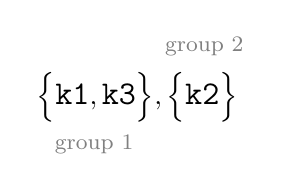
\begin{tikzpicture}
    \node at (0,0.6) {$\Big\lbrace \texttt{\large k1}, \texttt{\large k3} \Big\rbrace,
\Big\lbrace \texttt{\large k2} \Big\rbrace$};
    \node[smallgraytext] at (-0.55,0) {group 1};
    \node[smallgraytext] at (0.85, 1.25) {group 2};
\end{tikzpicture}
\end{figure}
\end{frame}

\begin{frame}[fragile]
A \texttt{UnionFind} stores \texttt{UnifNode} objects and supports the following operations:\\~\\
\begin{itemize}

\item \highlight{\texttt{make\_set}} \\
\graytext{creates a new set containing an object}\\[-1mm]
\begin{lstlisting}[style=mypython]
make_set(key: Key, obj: Object) -> Optional[UnifNode]
\end{lstlisting}

\item \highlight{\texttt{find\_set}} \\
\graytext{finds the representative of \texttt{key} (with path compression)}\\[-1mm]
\begin{lstlisting}[style=mypython]
find_set(key: Key) -> Optional[UnifNode]
\end{lstlisting}

\item \highlight{\texttt{union\_sets}} \\
\graytext{unions the representatives of \texttt{key1} and \texttt{key2} (by rank)}\\[-1mm]
\begin{lstlisting}[style=mypython]
union_sets(key1: Key, key2: Key) -> Optional[UnifNode]
\end{lstlisting}
\end{itemize}
\end{frame}

\begin{frame}{Union-Finds (via Forests)}
\begin{center}
    \Large \highlight{\texttt{UnionFind}} \\[1mm]
    \normalsize\color{gray} (via Forests)
\end{center}
\end{frame}


\begin{frame}
Suppose the set $\left\lbrace \texttt{a}, \dots, \texttt{g} \right\rbrace$, is divided into three groups:\\[4mm]
\begin{minipage}{0.33\textwidth}
\begin{center}
$\left\lbrace \texttt{a}, \texttt{b}, \texttt{g} \right\rbrace$
\end{center}
\begin{figure}
\centering
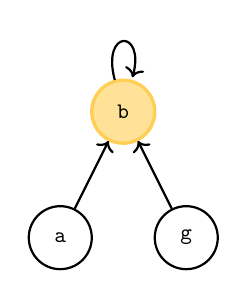
\begin{tikzpicture}[scale=0.8, transform shape]

\node[newnode] (tB) at (0,2) {\texttt{b}};
\node[defaultnode] (tA) at (-1,0) {\texttt{a}};
\node[defaultnode] (tG) at (1,0) {\texttt{g}};

\draw[defaultnode, <-] (tB) edge (tA);
\draw[defaultnode, <-] (tB) edge (tG);
\draw[defaultnode, <-] (tB) edge[loop above] (tB);

\end{tikzpicture}
\end{figure}
\end{minipage}%
\begin{minipage}{0.33\textwidth}
\begin{center}
$\left\lbrace \texttt{c}, \texttt{e}, \texttt{h} \right\rbrace$
\end{center}
\begin{figure}
\centering
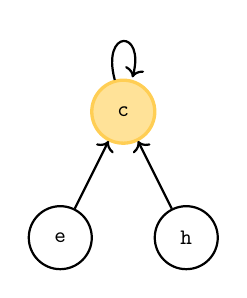
\begin{tikzpicture}[scale=0.8]
\node[newnode] (tC) at (0,2) {\texttt{c}};
\node[defaultnode] (tE) at (-1,0) {\texttt{e}};
\node[defaultnode] (tH) at (1,0) {\texttt{h}};


\draw[defaultnode, <-] (tC) edge (tE);
\draw[defaultnode, <-] (tC) edge (tH);
\draw[defaultnode, <-] (tC) edge[loop above] (tC);

\end{tikzpicture}
\end{figure}
\end{minipage}%
\begin{minipage}{0.33\textwidth}
\begin{center}
$\left\lbrace \texttt{d}, \texttt{f} \right\rbrace$
\end{center}
\begin{figure}
\centering
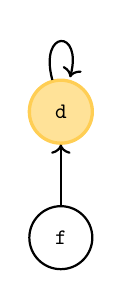
\begin{tikzpicture}[scale=0.8]

\node[newnode] (tD) at (0,2) {\texttt{d}};
\node[defaultnode] (tF) at (0,0) {\texttt{f}};

\draw[defaultnode, <-] (tD) edge (tF);
\draw[defaultnode, <-] (tD) edge[loop above] (tD);
\end{tikzpicture}
\end{figure}
\end{minipage}
\\~\\[2mm]
We represent each set as a tree, with the root being its \highlight{\textbf{representative}}.
\end{frame}

\begin{frame}[fragile]
\begin{thmboxtop}
\highlight{\texttt{UnionFind}} \\
\graytext{(via Forests)}
\begin{lstlisting}[style=mypython]
class UnifNode:
# attributes
    # the key of this node
    key: Key

    # the object of this node
    obj: Object

    # the parent of this node
    pnt: Optional[UnifNode]
\end{lstlisting}
\end{thmboxtop}    
\end{frame}

\begin{frame}[fragile]
\begin{thmboxbot}
\begin{lstlisting}[style=mypython]
class UnionFind:
# attributes
    # nodes in a forest of trees (representing disjoint sets)
    nodes: Dict[Key, UnifNode]
    
    # the number of nodes
    size: Integer

# functions
    ...
\end{lstlisting}
\end{thmboxbot}    
\end{frame}

\begin{frame}
\texttt{make\_set} creates a new node serving as its own representative.

\begin{center}
\highlight{\textbf{make set}} \\
\footnotesize\color{gray} \texttt{make\_set(a),...,make\_set(h)}
\end{center}
\begin{figure}
\centering
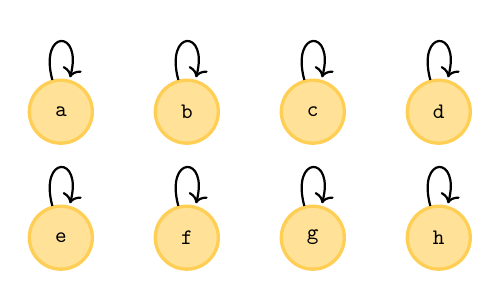
\begin{tikzpicture}[scale=0.8]
\node[newnode] (tA) at (0,0) {\texttt{a}};
\node[newnode] (tB) at (2,0) {\texttt{b}};
\node[newnode] (tC) at (4,0) {\texttt{c}};
\node[newnode] (tD) at (6,0) {\texttt{d}};
\node[newnode] (tE) at (0,-2) {\texttt{e}};
\node[newnode] (tF) at (2,-2) {\texttt{f}};
\node[newnode] (tG) at (4,-2) {\texttt{g}};
\node[newnode] (tH) at (6,-2) {\texttt{h}};

\draw[defaultnode, <-] (tA) edge[loop above] (tA);
\draw[defaultnode, <-] (tB) edge[loop above] (tB);
\draw[defaultnode, <-] (tC) edge[loop above] (tC);
\draw[defaultnode, <-] (tD) edge[loop above] (tD);
\draw[defaultnode, <-] (tE) edge[loop above] (tE);
\draw[defaultnode, <-] (tF) edge[loop above] (tF);
\draw[defaultnode, <-] (tG) edge[loop above] (tG);
\draw[defaultnode, <-] (tH) edge[loop above] (tH);

\end{tikzpicture}
\end{figure}
\begin{center}
\graytext{each node is its own representative}
\end{center}
\end{frame}

\begin{frame}[fragile]
\begin{proofbox}
\begin{lstlisting}[style=mypython]
def make_set(self: UnionFind, key: Key, obj: Object) -> Optional[UnifNode]:
    self.nodes.insert(key, obj)
    self.size += 1
    return self.nodes.get(key)
\end{lstlisting}
\end{proofbox}
\end{frame}

\begin{frame}
\texttt{find\_set} follows the parents to return the representative of the node's set.
\begin{center}
\highlight{\textbf{find}} \\
\footnotesize\color{gray} \texttt{find\_set(h)}
\end{center}
\begin{center}
\begin{figure}
\centering
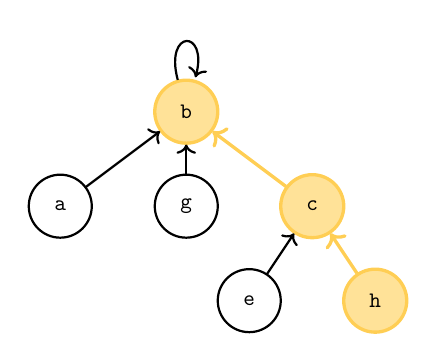
\begin{tikzpicture}[scale=0.8]
\node[newnode] (tB) at (0,1.5) {\texttt{b}};
\node[defaultnode] (tA) at (-2,0) {\texttt{a}};
\node[defaultnode] (tG) at (0,0) {\texttt{g}};
\node[newnode] (tC) at (2,0) {\texttt{c}};
\node[defaultnode] (tE) at (1,-1.5) {\texttt{e}};
\node[newnode] (tH) at (3,-1.5) {\texttt{h}};


\draw[defaultnode, <-] (tB) edge (tA);
\draw[defaultnode, <-] (tB) edge (tG);
\draw[defaultnode, <-] (tB) edge[loop above] (tB);
\draw[newnode, <-] (tB) edge (tC);
\draw[defaultnode, <-] (tC) edge (tE);
\draw[newnode, <-] (tC) edge (tH);

\end{tikzpicture}
\end{figure}
\end{center}
\begin{center}
\graytext{\texttt{h}'s parent is \texttt{c}, \texttt{c}'s parent is \texttt{b}; \\ \texttt{b} is the representative since it is its own parent}
\end{center}
\end{frame}

\begin{frame}[fragile]
\begin{proofbox}
\begin{lstlisting}[style=mypython]
def find_set(self: UnionFind, key: Key) -> Optional[UnifNode]:
    node = self.nodes.get(key)
    if node is None:
        return None
    if node.pnt.key is key
        return node
    return self.find_set(node.pnt.key)
\end{lstlisting}
\end{proofbox}
\end{frame}

\begin{frame}
\texttt{union\_sets} takes the representative of one set and makes its parent the representative of the other.
\begin{center}
\highlight{\textbf{union}} \\
\footnotesize\color{gray} \texttt{union\_set(h,a)}
\end{center}
\begin{center}
\begin{figure}
\centering
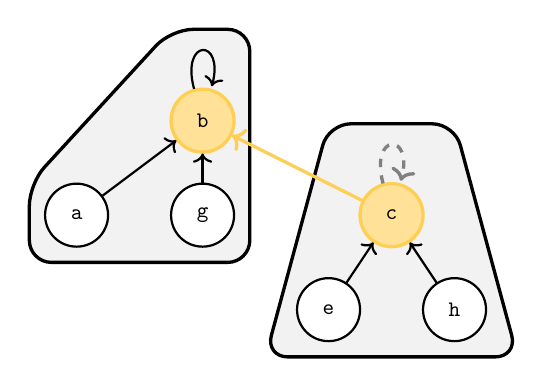
\begin{tikzpicture}[scale=0.8]
\filldraw[very thick, draw=black, fill=lightgray!20, rounded corners=8pt]
(-0.5,2.95) -- (0.75,2.95) -- (0.75,-0.75) -- (-2.75,-0.75) -- (-2.75,0.5) -- cycle;

\begin{scope}[xshift=3cm, yshift=1cm]
\filldraw[very thick, draw=black, fill=lightgray!20, rounded corners=8pt] (-1,0.45) -- (1,0.45) -- (2,-3.25) -- (-2,-3.25) -- cycle;    
\end{scope}

\node[newnode] (tB) at (0,1.5) {\texttt{b}};
\node[defaultnode] (tA) at (-2,0) {\texttt{a}};
\node[defaultnode] (tG) at (0,0) {\texttt{g}};
\node[newnode] (tC) at (3,0) {\texttt{c}};
\node[defaultnode] (tE) at (2,-1.5) {\texttt{e}};
\node[defaultnode] (tH) at (4,-1.5) {\texttt{h}};

\draw[defaultnode, <-] (tB) edge (tA);
\draw[defaultnode, <-] (tB) edge (tG);
\draw[defaultnode, <-] (tB) edge[loop above] (tB);
\draw[newnode, <-] (tB) edge (tC);
\draw[defaultnode, <-] (tC) edge (tE);
\draw[defaultnode, <-] (tC) edge (tH);
\draw[very thick, gray, <-, dashed] (tC) edge[loop above] (tC);
\end{tikzpicture}
\end{figure}
\end{center}
\begin{center}
\graytext{the parent of \texttt{h}'s representative (\texttt{c}) becomes \texttt{a}'s representative (\texttt{b})}
\end{center}

\end{frame}


\begin{frame}[fragile]
\begin{proofbox}
\begin{lstlisting}[style=mypython]
def union_sets(self: UnionFind, key1: Key, key2: Key):
    rep1 = self.find_set(key1)
    rep2 = self.find_set(key2)

    if rep1 is None or rep2 is None:
        return
    if rep1 is not rep2:
        rep1.pnt = rep2 # or the other way
\end{lstlisting}
\end{proofbox}
\end{frame}

\begin{frame}
\begin{center}
\begin{table}
\begin{tabular}{@{} r | l @{} }
\highlight{\textbf{Property}} & \\[1mm]\hline
\multirow{1}{*}{Time Complexity} & \\
\color{gray}\footnotesize\texttt{make\_set} & \color{gray}\footnotesize $O(1)$\\[1mm]
\color{gray}\footnotesize\texttt{find\_set} & \color{gray}\footnotesize $O(S)$ \\[1mm]
\color{gray}\footnotesize\texttt{union\_sets} & \color{gray}\footnotesize $O(S)$\\[1mm]
Space Complexity & $O(S)$
\end{tabular}
\end{table}
\end{center}
\begin{center}
\footnotesize\color{gray} properties of the \texttt{UnionFind} data-structure
\end{center}
\renewcommand\thefootnote{}\footnotetext{\color{gray} Assumptions: $S = \texttt{UnionFind.size}$}
\end{frame}

\begin{frame}
\texttt{union\_sets} should attach the shorter tree to the longer one.
\begin{center}
\highlight{\textbf{union}} \\
\footnotesize\color{gray} \texttt{union\_sets(g,f)} by height
\end{center}
\begin{figure}
\centering
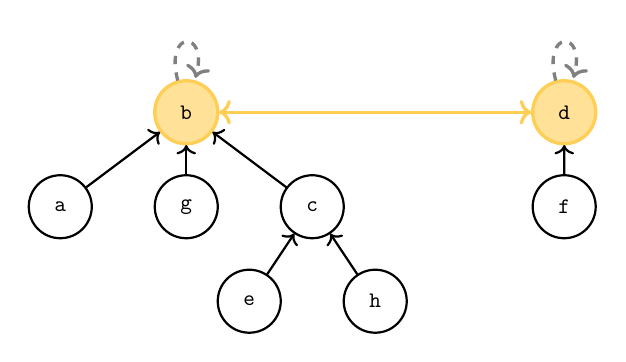
\begin{tikzpicture}[scale=0.8]
\node[newnode] (tB) at (0,1.5) {\texttt{b}};
\node[defaultnode] (tA) at (-2,0) {\texttt{a}};
\node[defaultnode] (tG) at (0,0) {\texttt{g}};
\node[defaultnode] (tC) at (2,0) {\texttt{c}};
\node[defaultnode] (tE) at (1,-1.5) {\texttt{e}};
\node[defaultnode] (tH) at (3,-1.5) {\texttt{h}};
\node[newnode] (tD) at (6,1.5) {\texttt{d}};
\node[defaultnode] (tF) at (6,0) {\texttt{f}};

\draw[defaultnode, <-] (tB) edge (tA);
\draw[defaultnode, <-] (tB) edge (tG);
\draw[very thick, gray, <-, dashed] (tB) edge[loop above] (tB);
\draw[defaultnode, <-] (tB) edge (tC);
\draw[defaultnode, <-] (tC) edge (tE);
\draw[defaultnode, <-] (tC) edge (tH);

\draw[defaultnode, <-] (tD) edge (tF);
\draw[very thick, gray, <-, dashed] (tD) edge[loop above] (tD);

\draw[newnode, <->] (tB) edge (tD);

\end{tikzpicture}
\end{figure}
\begin{center}
    \footnotesize\color{gray} \texttt{d} should be attached to \texttt{b} to minimize the tree height
\end{center}
\end{frame}

\begin{frame}[fragile]
Computing the exact height of the resulting tree after a \texttt{union\_sets} operation is hard since it would require traversing the entire tree.
\\~\\
Thus, we maintain an upper-bound on the height (called the rank) using an attribute in the \texttt{UnifNode} class:
\begin{lstlisting}[style=mypython]
rank: Integer
\end{lstlisting}
where \texttt{rank} contains an upper-bound on the height of the node.
\end{frame}

\begin{frame}
\begin{thmbox}
The \highlight{\textbf{rank}} of a tree is a positive integer defined such that:
\begin{itemize}
\item a tree consisting of a single node has rank $1$
\item when \texttt{union\_sets} is performed on two trees with the same rank, the rank of the resulting tree is increased by one
\end{itemize}
\end{thmbox}
\end{frame}

\begin{frame}
\texttt{union\_sets} should attach the the lower ranked tree to the higher one.
\begin{center}
\highlight{\textbf{union}} \\
\footnotesize\color{gray} \texttt{union\_sets(g,f)} by rank
\end{center}
\begin{figure}
\centering
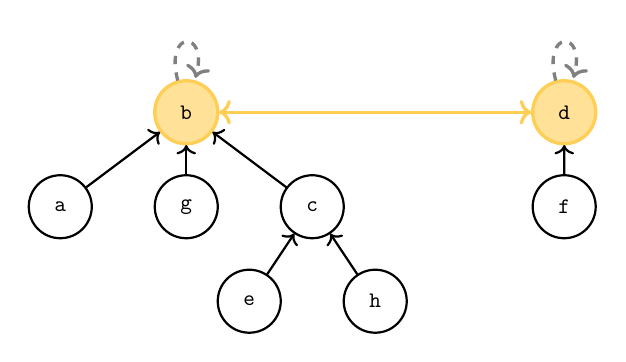
\begin{tikzpicture}[scale=0.8]
\node[newnode] (tB) at (0,1.5) {\texttt{b}};
\node[defaultnode] (tA) at (-2,0) {\texttt{a}};
\node[defaultnode] (tG) at (0,0) {\texttt{g}};
\node[defaultnode] (tC) at (2,0) {\texttt{c}};
\node[defaultnode] (tE) at (1,-1.5) {\texttt{e}};
\node[defaultnode] (tH) at (3,-1.5) {\texttt{h}};
\node[newnode] (tD) at (6,1.5) {\texttt{d}};
\node[defaultnode] (tF) at (6,0) {\texttt{f}};


\draw[defaultnode, <-] (tB) edge (tA);
\draw[defaultnode, <-] (tB) edge (tG);
\draw[very thick, gray, <-, dashed] (tB) edge[loop above] (tB);
\draw[defaultnode, <-] (tB) edge (tC);
\draw[defaultnode, <-] (tC) edge (tE);
\draw[defaultnode, <-] (tC) edge (tH);

\draw[defaultnode, <-] (tD) edge (tF);
\draw[very thick, gray, <-, dashed] (tD) edge[loop above] (tD);

\draw[newnode, <->] (tB) edge (tD);

\end{tikzpicture}
\end{figure}
\begin{center}
    \footnotesize\color{gray} \texttt{d} (rank 2) should be attached to \texttt{b} (rank 3)
\end{center}
\end{frame}

\begin{frame}[fragile]
\begin{proofbox}
\begin{lstlisting}[style=mypython]
def union_sets(self: UnionFind, key1: Key, key2: Key):
    # with ranking...
    rep1 = self.find_set(key1)
    rep2 = self.find_set(key2)

    if rep1 is None or rep2 is None:
        return
    if rep1 is not rep2:
        # ranks are different
        if rep1.rank is not rep2.rank:
            if rep1.rank < rep2.rank:
                rep1.pnt = rep2
            else:
                rep2.pnt = rep1
        # ranks are same
        else:
            rep2.pnt = rep1
            rep1.rank += 1
\end{lstlisting}
\end{proofbox}

\end{frame}


\begin{frame}
\texttt{find\_set} should attach each non-representative to the representative
\begin{center}
\highlight{\textbf{find}} \\
\footnotesize\color{gray} \texttt{find\_set(i)} with compression
\end{center}
\vspace{-3mm}
\begin{figure}
\centering
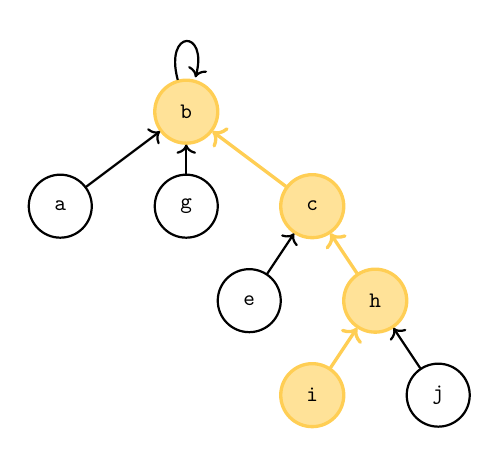
\begin{tikzpicture}[scale=0.8]
\node[newnode] (tB) at (0,1.5) {\texttt{b}};
\node[defaultnode] (tA) at (-2,0) {\texttt{a}};
\node[defaultnode] (tG) at (0,0) {\texttt{g}};
\node[newnode] (tC) at (2,0) {\texttt{c}};
\node[defaultnode] (tE) at (1,-1.5) {\texttt{e}};
\node[newnode] (tH) at (3,-1.5) {\texttt{h}};
\node[newnode] (tI) at (2,-3) {\texttt{i}};
\node[defaultnode] (tJ) at (4,-3) {\texttt{j}};


\draw[defaultnode, <-] (tB) edge (tA);
\draw[defaultnode, <-] (tB) edge (tG);
\draw[defaultnode, <-] (tB) edge[loop above] (tB);
\draw[newnode, <-] (tB) edge (tC);
\draw[defaultnode, <-] (tC) edge (tE);
\draw[newnode, <-] (tC) edge (tH);

\draw[newnode, <-] (tH) edge (tI);
\draw[defaultnode, <-] (tH) edge (tJ);

\end{tikzpicture}
\end{figure}
\begin{center}
\graytext{\texttt{i}, \texttt{h}, and \texttt{c} should all get attached to \texttt{b}}
\end{center}
\end{frame}


\begin{frame}
\begin{center}
\highlight{\textbf{find}} \\
\footnotesize\color{gray} \texttt{find\_set(i)} with compression
\end{center}
\vspace{-3mm}
\begin{figure}
\centering
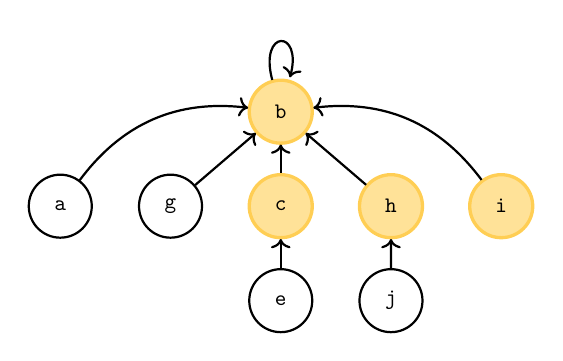
\begin{tikzpicture}[scale=0.8]
\node[newnode] (tB) at (0,1.5) {\texttt{b}};
\node[defaultnode] (tA) at (-3.5,0) {\texttt{a}};
\node[defaultnode] (tG) at (-1.75,0) {\texttt{g}};
\node[newnode] (tC) at (0,0) {\texttt{c}};
\node[defaultnode] (tE) at (0,-1.5) {\texttt{e}};
\node[newnode] (tH) at (1.75,0) {\texttt{h}};
\node[newnode] (tI) at (3.5,0) {\texttt{i}};
\node[defaultnode] (tJ) at (1.75,-1.5) {\texttt{j}};


\draw[defaultnode, <-] (tB) edge[bend right] (tA);
\draw[defaultnode, <-] (tB) edge (tG);
\draw[defaultnode, <-] (tB) edge[loop above] (tB);
\draw[defaultnode, <-] (tB) edge (tC);
\draw[defaultnode, <-] (tC) edge (tE);
\draw[defaultnode, <-] (tB) edge (tH);

\draw[defaultnode, <-] (tB) edge[bend left] (tI);
\draw[defaultnode, <-] (tH) edge (tJ);

\end{tikzpicture}
\end{figure}
\begin{center}
\graytext{\;}
\end{center}
\end{frame}

\begin{frame}[fragile]
\begin{proofbox}
\begin{lstlisting}[style=mypython]
def find_set(self: UnionFind, key: Key) -> Optional[UnifNode]:
    # with compression...
    node = self.nodes.get(key)
    if node is None:
        return
    if node.pnt.key is key:
        return self.nodes.get(key)    
    rep = self.find_set(node.pnt.key)
    node.pnt = rep
    return rep
\end{lstlisting}
\end{proofbox}
\end{frame}

\begin{frame}
\begin{center}
\begin{table}
\begin{tabular}{@{} r | l @{} }
\highlight{\textbf{Property}} & \\[1mm]\hline
\multirow{1}{*}{Time Complexity} & \\
\color{gray}\footnotesize\texttt{make\_set} & \color{gray}\footnotesize $O(1)$\\[1mm]
\color{gray}\footnotesize\texttt{find\_set} & \color{gray}\footnotesize $\hat{O}(1)$ \\[1mm]
\color{gray}\footnotesize\texttt{union\_sets} & \color{gray}\footnotesize $\hat{O}(1)$\\[1mm]
Space Complexity & $O(S)$
\end{tabular}
\end{table}
\end{center}
\begin{center}
    \footnotesize\color{gray} properties of the \texttt{UnionFind} data-structure \\ with ranking and compression
\end{center}
\renewcommand\thefootnote{}\footnotetext{\color{gray} Assumptions: $S = \texttt{UnionFind.size}$}
\end{frame}


\end{document}